\usetikzlibrary{plotmarks}

\begin{figure}[htbp]
\centering
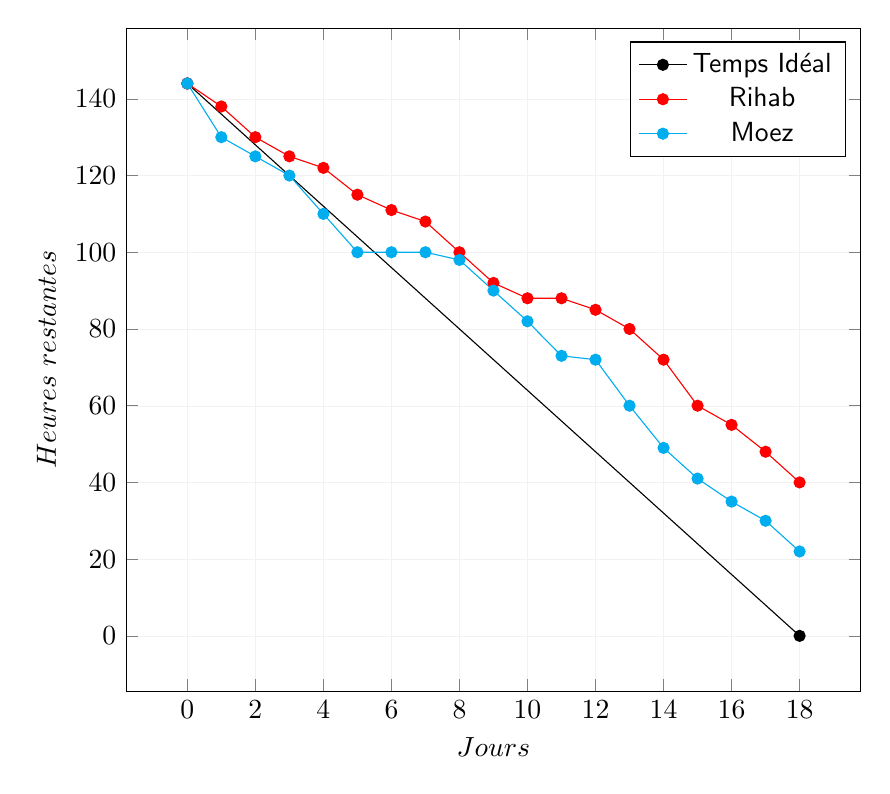
\begin{tikzpicture}[y=.1cm, x=.7cm,font=\sffamily]
\begin{axis}[
xlabel=$Jours$,
ylabel=$Heures\ restantes$,
grid=both,
grid style={line width=.1pt, draw=gray!10},
width=0.9\textwidth,
height=10cm,
%major grid style={line width=.2pt,draw=gray!50},
]
\addplot[color=black,mark=*] coordinates {
        (0,144)
        (18,0)
    };
    \addlegendentry{Temps Idéal}

    \addplot[mark=*,red] plot coordinates {
        (0, 144)
        (1, 138)
        (2, 130)
        (3, 125)
        (4, 122)
        (5, 115)
        (6, 111)
        (7, 108)
        (8, 100)
        (9, 92)
        (10, 88)
        (11, 88)
        (12, 85)
        (13, 80)
        (14, 72)
        (15, 60)
        (16, 55)
        (17, 48)
        (18, 40)
       
    };
    \addlegendentry{Rihab}
      \addplot[mark=*,cyan] plot coordinates {
        (0, 144)
        (1, 130)
        (2, 125)
        (3, 120)
        (4, 110)
        (5, 100)
        (6, 100)
        (7, 100)
        (8, 98)
        (9, 90)
        (10, 82)
        (11, 73)
        (12, 72)
        (13, 60)
        (14, 49)
        (15, 41)
        (16, 35)
        (17, 30)
        (18, 22)
       
    };
    \addlegendentry{Moez}
\end{axis}
\end{tikzpicture}
\caption{Graphique d'avancement - Itération 2}
\end{figure}
